\section{El elemento en su posición}

\begin{frame}{El elemento en su posición}
\begin{description}
 \item[Entrada:] Vector ordenado \texttt{v} (sin repetidos) y su tamaño \texttt{n}
 \item[Salida:] Entero no negativo que indica el $i$ tal que $v[i]=i$ en caso de que exista o $-1$ en otro caso
\end{description}
\end{frame}

\subsection{Algoritmos}

\begin{frame}[fragile]{Algoritmo obvio}
Recorre cada elemento y comprueba si $v[i] = i$:
\lstinputlisting[firstline=23, lastline=28]{cpps/posicion.cpp}
\textbf{Eficiencia:} $O(n)$.
\end{frame}

\begin{frame}[fragile]{Algoritmo recursivo}
\lstinputlisting[firstline=60, lastline=72]{cpps/posicion.cpp}
\note{\texttt{ajuste}: ajusta la comprobación en función de la posición.
El caso base utiliza el algoritmo obvio ajustado.}
\end{frame}

\begin{frame}{Casos del algoritmo}
El algoritmo considera \textbf{3} casos:
\begin{itemize}
  \item El elemento medio está en su posición
  \item $m < v[m]$. Basta comprobar el lado izquierdo:
  \[v[m + k] \geq v[m]+k>m+k\]
  \item $m > v[m]$. Basta comprobar el lado derecho:
  \[v[m - k] \leq v[m] -k < m - k\]
\end{itemize}
\end{frame}

\begin{frame}{Eficiencia teórica}
\[T(n) = \begin{cases} T(n/2) + O(1) & \mbox{si } n > 3 \\
O(1) & \mbox{si } n \leq 3 \end{cases}\]
\textbf{Eficiencia:} $O(\log(n))$.
\end{frame}

\begin{frame}[fragile]{Versión no recursiva}
\lstinputlisting[firstline=87, lastline=101]{cpps/posicion.cpp}
\textbf{Eficiencia:} $O(\log(n))$
\end{frame}

\subsection{Determinación del umbral}

%% TODO: (Antonio) Estudio del umbral ¿algo más?

\begin{frame}[fragile]{Umbral (tablas)}
\pgfplotstableread{dats/comp_umbral_posicion/posicion_t.dat}\posObvioCompUmbral
\pgfplotstableread{dats/comp_umbral_posicion/posicion_1.dat}\posDyVUmbralOne
\pgfplotstableread{dats/comp_umbral_posicion/posicion_1_umbral_2.dat}\posDyVUmbralTwo
\pgfplotstableread{dats/comp_umbral_posicion/posicion_1_umbral_3.dat}\posDyVUmbralThree
\pgfplotstableread{dats/comp_umbral_posicion/posicion_1_umbral_4.dat}\posDyVUmbralFour
\pgfplotstableread{dats/comp_umbral_posicion/posicion_1_umbral_5.dat}\posDyVUmbralFive
\pgfplotstablecreatecol[copy column from table={\posDyVUmbralOne}{[index] 1}] {par1} {\posObvioCompUmbral}
\pgfplotstablecreatecol[copy column from table={\posDyVUmbralTwo}{[index] 1}] {par2} {\posObvioCompUmbral}
\pgfplotstablecreatecol[copy column from table={\posDyVUmbralThree}{[index] 1}] {par3} {\posObvioCompUmbral}
\pgfplotstablecreatecol[copy column from table={\posDyVUmbralFour}{[index] 1}] {par4} {\posObvioCompUmbral}
\pgfplotstablecreatecol[copy column from table={\posDyVUmbralFive}{[index] 1}] {par5} {\posObvioCompUmbral}

\resizebox{\linewidth}{!}{
\pgfplotstabletypeset[
display columns/0/.style={column name=Tamaño},
display columns/1/.style={column name=Obvio},
display columns/2/.style={column name=Umbral 1},
display columns/3/.style={column name=Umbral 2},
display columns/4/.style={column name=Umbral 3},
display columns/5/.style={column name=Umbral 4},
display columns/6/.style={column name=Umbral 5},
]{\posObvioCompUmbral}
}
\end{frame}

\begin{frame}{Umbral (gráficas)}
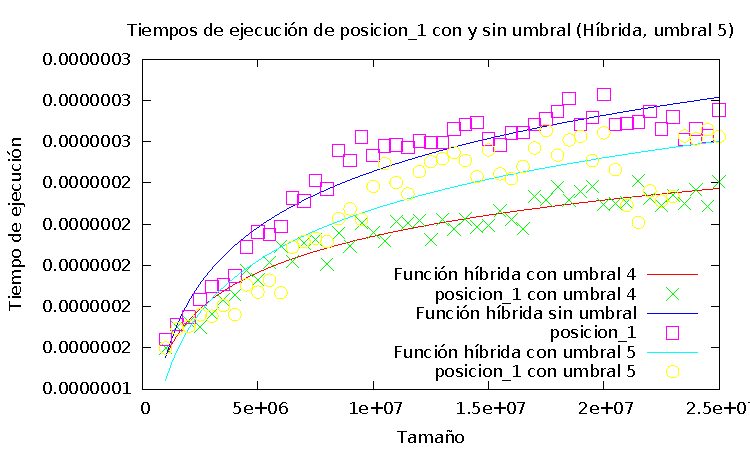
\includegraphics[width=\textwidth]{img/posicion_1_comparativa_umbral2.pdf}
\end{frame}

\begin{frame}{Umbral (gráficas)}
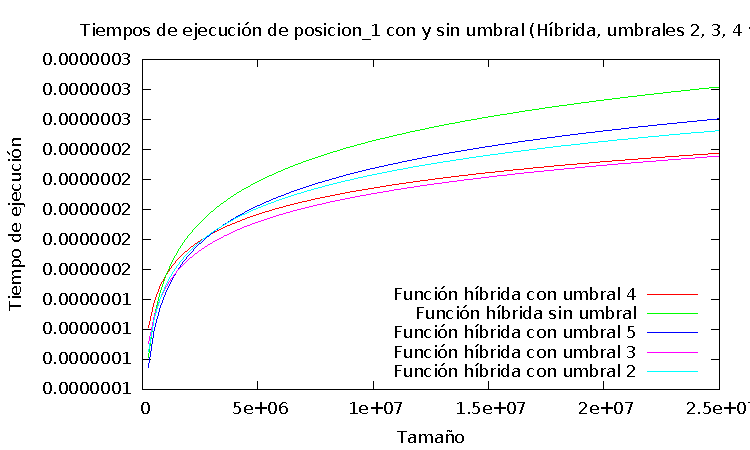
\includegraphics[width=\textwidth]{img/posicion_1_comparativa_umbral5.pdf}
\note{Como poner los 5 umbrales y sus híbridas haría que la gráfica fuera un poco caótica, hemos decidido poner una gráfica solo con las híbridas de los algoritmos, para que se vea la tendencia de los tiempos, que es lo que importa.}
\end{frame}

\begin{frame}{Umbral - Tamaño - Tiempo}
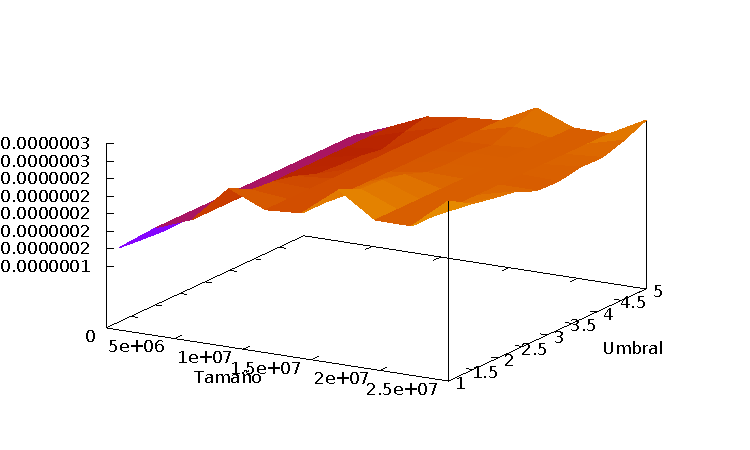
\includegraphics[width=\textwidth]{img/umbral_posicion.pdf}
\end{frame}

\subsection{Eficiencia empírica de los algoritmos}

\begin{frame}[fragile]{Eficiencia empírica (tabla)}
\pgfplotstableread{dats/comp_umbral_posicion/posicion_t.dat}\posObvio
\pgfplotstableread{dats/comp_umbral_posicion/posicion_1.dat}\posDyV
%\pgfplotstableread{dats/comp_umbral_posicion/posicion_2.dat}\posDyVTwo
\pgfplotstablecreatecol[copy column from table={\posDyV}{[index] 1}] {par1} {\posObvio}
%\pgfplotstablecreatecol[copy column from table={\posDyVTwo}{[index] 1}] {par2} {\posObvio}
\resizebox{\linewidth}{!}{
\pgfplotstabletypeset[
display columns/0/.style={column name=Tamaño},
display columns/1/.style={column name=Algoritmo Obvio},
display columns/2/.style={column name=Algoritmo DyV (rec)},
%display columns/3/.style={column name=Algoritmo DyV (no rec)},
]{\posObvio}
}

\note{Aunque los algoritmos son rápidos para tamaños grandes, las funciones auxiliares utilizadas para la generación de muestras aleatorias que permitan medir el tiempo han dificultado la obtención de los datos. Los datos obtenidos pueden verse en la tabla.}
\end{frame}

\begin{frame}{Ajuste de las funciones (tabla)}
%% TODO: (¿?) Ajustes de las funciones
\end{frame}

\begin{frame}{Ajuste de las funciones (tabla)}
%% TODO: (Antonio) Gráfica con todos los algoritmos
\end{frame}

\subsection{Vectores con elementos repetidos}

En el caso de que tengamos elementos repetidos el razonamiento realizado para justificar el algoritmo divide y vencerás no es válido, y es sencillo encontrar ejemplos de vectores con elementos en su posición para los cuales nuestro algoritmo no funciona.

\begin{frame}{El algoritmo falla}
%% TODO: Poner bonico
\note{$v = [1,2,2]$. $1 <v[1]$, por lo que nuestro algoritmo comprobaría sólo el lado izquierdo ($[1]$) y no encontraría el elemento en la posición 2, que está en su posición.}
\end{frame}

\begin{frame}[fragile]{Algoritmo}
\resizebox{0.6\linewidth}{!}{
\lstinputlisting[firstline=111, lastline=135]{cpps/posicion.cpp}}
\note{
Casi logarítmico cuando hay un elemento en su posición, y peor que lineal cuando no se encuentra.
Como en una distribución uniforme sobre el rango de elementos en los que trabajamos la probabilidad de que un elemento caiga en su posición es bastante baja, por mucho que a veces sea logarítmico, no compensa las veces que es peor que lineal.}
\end{frame}

\begin{frame}{Comparación (tablas)}
  %%TODO: Comparación
\end{frame}

\begin{frame}{Comparación (gráficas)}
  %%TODO: Comparación
\end{frame}
